\section{Spectraèdres réels}

\newcommand\ssp{symétrique semi-définie positive}
\newcommand\ssps{symétriques semi-définies positives}
\newcommand\Ssp{Symétrique semi-définie positive}
\newcommand\Ssps{Symétriques semi-définies positives}

\subsection{définiion?}
\todo{trouver un nom}

\begin{definition}
	On appelle \emph{matrice symétrique semi-définie positive} toute matrice réelle symétriques et à valeurs propres positives ou nulles.
	On notera $\mathcal{S}_n^+\left(\mathbb{R}\right) $ l'ensemble de telles matrices et $M \succeq 0$ le fait que $M \in \mathcal{S}_n^+\left(\mathbb{R}\right)$.
\end{definition}

\begin{remarque}
	On remarquera que demander la symétrie, n'est, dans le cas réel, qu'un moyen de s'assurer d'obtenir des valeurs propres réelles grâce au théorème spectral.
\end{remarque}
\begin{propriete}
	L'ensemble $\mathcal{S}_n^+\left( \mathbb{R} \right) $ est un cône convexe fermé.
\end{propriete}

\begin{definition}
	On appelle \emph{spectraèdre} l'intersection de $\mathcal{S}_n^+\left(\mathbb{R}\right)$ avec un espace affine $\mathcal{L}$ de $\mathcal{S}_n\left(\mathbb{R}\right)$.
\end{definition}

En écrivant l'hyperplan $\mathcal{L}$ de $\mathcal{S}_n^+\left(\mathbb{R}\right)$ sous sa forme paramétrique \textit{i.e.} comme l'ensemble des matrices de la forme $A_0 + x_1 A_1 + \ldots x_s A_s$ pour $A_0,\ldots, A_s$ des matrices symétriques fixées on peut définir le spéctraèdre $\mathcal{S} = \mathcal{L} \cap \mathcal{S}_n^+\left(\mathbb{R}\right)$ comme
$\mathcal{S} = \{A := A_0 + x_1A_1 + \ldots + x_s A_s | A \succeq 0, (x_1,\ldots,x_s) \in \mathbb{R}^s\}$. On identifie alors souvent ce dernier à sa préimage dans $\mathbb{R}^s$
$S = \{(x_1,\ldots,x_s) \in \mathbb{R}^s | A_0+ x_1A_1 + \ldots+ x_s A_s \succeq 0 \}. $

\simone{
  \begin{ex} Un exemple celèbre de spectraèdre est l'ensemble des matrices symétrique semi-définie positives
    avec diagonale $(1,1,1)$:
    $$
    S = \left\{
    \begin{pmatrix} x_1 \\ x_2 \\ x_3 \end{pmatrix} \in \mathbb{R}^3 |
    A:=\begin{pmatrix} 1 & x_1 & x_2 \\ x_1 & 1 & x_3 \\ x_2 & x_3 & 1 \end{pmatrix} \succeq 0
    \right\}.
    $$
    La surface algébrique définie par $\det A(x_1,x_2,x_3) = 0$ est dite {\it cubique de Cayley} (\ref{cayley}).
    %Le spectraèdre $S$ est souvent appélé {\it samosa} et peut être obtenu comme {\it dérivée au sens de Renegar} du tetraèdre régulier \cite{sanyal}.
    Les quatres points singuliers correspondent à quatre matrices semi-définies positives de rang un ; les autres points de la surface, correspondent à des matrices de rang deux (semi-définies si sur la frontière du spectraèdre, avec au moins une valeure propre négative autrement) ; enfin, les matrices à l'intérieur du spectraèdre sont définies positives (toutes valeurs singulières strictement positives).
    \begin{figure}[!ht]
      \centering
      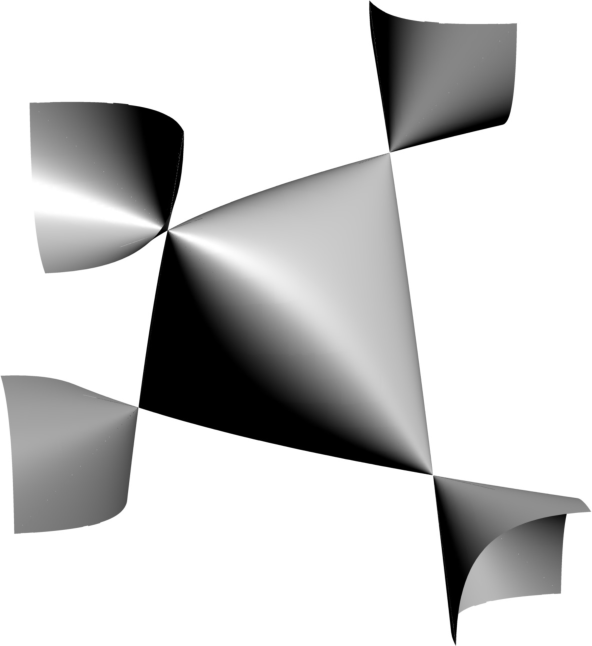
\includegraphics[scale=0.3]{figures/cayley.pdf}
      \caption{Cubique de Cayley}
      \label{cayley}
    \end{figure}
  \end{ex}
}

\subsection{Programmation semi-définie}

On appelle alors \emp{programmation semi-définie} le problème d'optimisation
consistant à minimiser une application linéaire sur un spéctraèdre que l'on formulera comme :
\begin{equation}
  \tag{PSD}
\begin{aligned}
  \text{Minimiser } & \simone{\left\langle c,x \right\rangle} \\
  \text{tel que }   & A_0 + \sum \limits_{i=1}^s x_{i}A_{i} \succeq 0
%	\begin{matrix}
%		\text{Minimiser } \simone{\left\langle c,x \right\rangle} \text{ tel que}\\
%		A_0 + \sum \limits_{i=1}^s x_{i}A_{i} \succeq 0
%	\end{matrix}
\end{aligned}
	\label{Psd} 
\end{equation}
pour $A_0,\ldots, A_s$ des matrices symétriques fixées, $c=(c_1,\ldots,c_s)$ un vecteur représentant le coût et $x \mapsto \left\langle c,x \right\rangle := c_1x_1+\cdots+c_sx_s$ le produit scalaire Euclidien. Le problème d'admissibilité associé au problème d'optimisation \eqref{Psd}, c'est-à-dire, la question si le spectraèdre $S = \{(x_1,\ldots,x_s) \in \mathbb{R}^s | A_0+ x_1A_1 + \ldots+ x_s A_s \succeq 0 \}$ est vide, est appelée \emp{inégalité matricielle linéaire (LMI)}.

En précision finie $\epsilon$, ce problème se résout en temps polynomial en la dimension de l'entrée (taille des matrices, nombre de variables, taille binaire des coefficients), en $\log(1/\epsilon)$ et $\log(R)$, où $R$ est une borne {\it a priori} sur la norme d'une solution. En arithmétique exacte, la complexité de la programmation semi-définie est un problème essentiellement ouvert, cf \cite[Sec.1.9]{deKlerk}, \cite{ramana1997exact,porkolab1997complexity} et \cite{henrion2016exact}.

Si à première vue ce problème peut sembler très spécifique il n'en est rien et de nombreux autres problèmes se rapportent à celui-ci. \simone{Par exemple, tout problème d'\simone{optimisation linéaire} est en particulier un problème SDP:

\begin{remarque} Un polyèdre est un spectraèdre; en particulier, l'optimisation linéaire est une sous-classe de l'optimisation semi-définie. En effet, soit $P = \{x \in \mathbb{R}^s | \ell_1(x) \geq 0, \ldots, \ell_d(x) \geq 0\}$ le polyèdre défini par les inégalités linéaires $\ell_1,\ldots,\ell_d$, et soit $D$ la matrice linéaire diagonale avec entrées $\ell_1,\ldots,\ell_d$. Alors $P$ est le spectraèdre défini par $D \succeq 0$.
\end{remarque}
}



%\todo{exemples: par }

%Le premier exemple étant que 
